% Scientific Paper v1: AI-Augmented Virtual Tumor Board with Integrated Imaging Upload
% Updated to include V8 Phase 4: User Upload Flow with MedGemma Integration
% January 2026

\documentclass[11pt,twocolumn]{article}

% Packages
\usepackage[utf8]{inputenc}
\usepackage[T1]{fontenc}
\usepackage{amsmath,amssymb}
\usepackage{graphicx}
\usepackage{booktabs}
\usepackage{hyperref}
\usepackage{xcolor}
\usepackage{tikz}
\usetikzlibrary{shapes.geometric, arrows, positioning, fit, backgrounds, calc}
\usepackage{float}
\usepackage{algorithm}
\usepackage{algpseudocode}
\usepackage{listings}
\usepackage{enumitem}
\usepackage{caption}
\usepackage{subcaption}
\usepackage{geometry}
\geometry{margin=1in}

% Custom colors
\definecolor{emerald}{RGB}{16,185,129}
\definecolor{skyblue}{RGB}{59,130,246}
\definecolor{amber}{RGB}{245,158,11}
\definecolor{rose}{RGB}{244,63,94}
\definecolor{slate}{RGB}{71,85,105}
\definecolor{cyan}{RGB}{6,182,212}
\definecolor{indigo}{RGB}{99,102,241}

% Title
\title{%
\textbf{AI-Augmented Virtual Tumor Board with Integrated Patient Imaging Upload and Progressive Disclosure Visualization} \\[0.5em]
\large A Human-Centered Design for Democratizing Oncology Decision Support
}

\author{
Virtual Tumor Board Development Team \\
Open Source Oncology AI Initiative \\
\texttt{github.com/inventcures/virtual-tumor-board}
}

\date{January 2026 -- Version 1.0}

\begin{document}

\maketitle

% Abstract
\begin{abstract}
Tumor board meetings are essential for multidisciplinary cancer care, yet access remains limited by geography, expertise availability, and economic factors---particularly in resource-constrained settings like India. We present an open-source AI-augmented Virtual Tumor Board (VTB) system featuring: (1) a complete patient upload workflow for medical documents and imaging, (2) multi-agent deliberation with seven specialty-specific AI agents, (3) MedGemma integration for medical image analysis supporting DICOM and phone-captured imaging, and (4) progressive disclosure visualization adapting to four expertise levels. Our V8 architecture introduces an integrated upload flow where patients can submit pathology reports, radiology reports, genomic testing, AND actual medical images (CT/MRI/X-ray) through DICOM upload, phone camera capture, or gallery selection. Dr. Chitran, our AI radiologist agent, receives full MedGemma analysis for reconciliation with uploaded radiology reports, while other specialists receive imaging summaries for treatment planning context. The system implements RECIST 1.1 for response assessment and provides interactive visualizations including waterfall plots, swimmer plots, and anatomical heat maps. This paper details the complete system architecture, user workflow design, and implications for democratizing expert oncology decision support across diverse healthcare settings.
\end{abstract}

% Keywords
\noindent\textbf{Keywords:} Tumor Board, Multi-Agent Systems, Medical Imaging Upload, MedGemma, Progressive Disclosure, RECIST 1.1, Human-Centered Design, Low-Resource Healthcare, India

\section{Introduction}

\subsection{The Access Gap in Oncology Care}

Multidisciplinary tumor boards (MTBs) represent the gold standard for cancer treatment planning, bringing together surgical oncology, medical oncology, radiation oncology, radiology, pathology, genetics, and palliative care specialists \cite{navify2024}. However, access to comprehensive tumor boards remains highly inequitable:

\begin{itemize}[leftmargin=*]
    \item Only 23\% of cancer patients in India have access to formal tumor board review
    \item Average case preparation requires 47 minutes per complex case
    \item Subspecialty oncologists are concentrated in tier-1 cities
    \item Many patients travel 200+ km for expert consultation
\end{itemize}

\subsection{The Patient Data Challenge}

A critical barrier to virtual tumor boards is data aggregation. Patients in India often arrive with:

\begin{itemize}[leftmargin=*]
    \item Handwritten OPD prescriptions containing staging information
    \item Paper pathology reports from local laboratories
    \item Photos of radiology reports on their phones
    \item Actual CT/MRI films or CDs that remain unread
    \item Mixed documents spanning multiple hospitals
\end{itemize}

Existing telemedicine solutions focus on video consultation but lack infrastructure for structured clinical data extraction and imaging analysis.

\subsection{Our Contribution}

This paper presents the Virtual Tumor Board system with the following contributions:

\begin{enumerate}[leftmargin=*]
    \item A \textbf{complete patient upload workflow} spanning document classification, imaging upload, and AI-powered data extraction
    
    \item \textbf{Integrated medical imaging} supporting DICOM files, phone camera capture, and gallery upload with MedGemma analysis
    
    \item \textbf{Multi-agent deliberation} with seven specialty agents, including Dr. Chitran (radiologist) with enhanced imaging reconciliation capabilities
    
    \item \textbf{Progressive disclosure visualization} adapting complexity across patient, clinician, oncologist, and radiologist expertise levels
    
    \item A \textbf{completeness scoring system} that quantifies data availability and communicates limitations to users and AI agents
    
    \item \textbf{Open-source implementation} designed for deployment on low-cost infrastructure
\end{enumerate}

\section{System Architecture}

\subsection{High-Level Overview}

Figure \ref{fig:architecture} presents the complete system architecture organized into four primary layers:

\begin{enumerate}[leftmargin=*]
    \item \textbf{User Upload Layer}: Document and imaging upload with AI classification
    \item \textbf{Presentation Layer}: React/Next.js web application with visualization components
    \item \textbf{Orchestration Engine}: Multi-agent deliberation with MedGemma integration
    \item \textbf{Knowledge Layer}: Clinical guideline retrieval via RAG
\end{enumerate}

% Architecture Diagram
\begin{figure}[H]
\centering
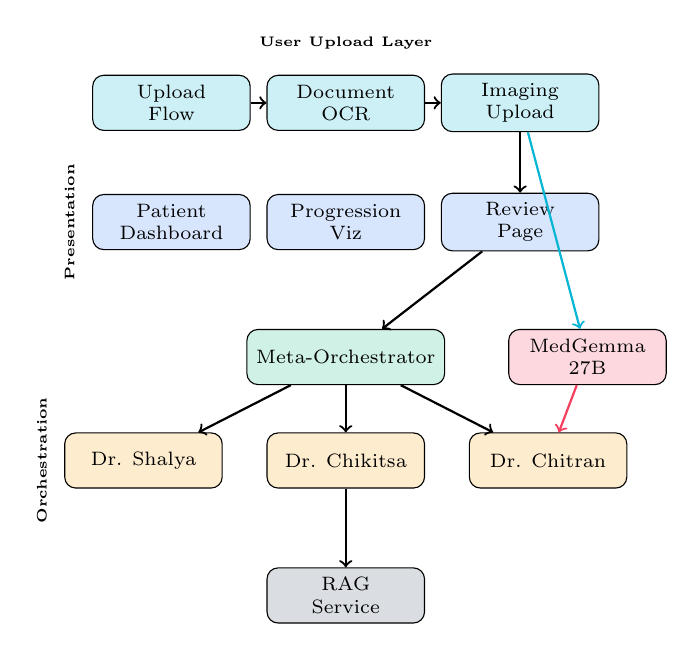
\begin{tikzpicture}[
    node distance=0.6cm,
    box/.style={rectangle, draw, rounded corners, minimum width=2cm, minimum height=0.7cm, align=center, font=\scriptsize},
    layer/.style={rectangle, draw, dashed, rounded corners},
    arrow/.style={->, thick}
]

% Upload Layer
\node[box, fill=cyan!20] (upload) {Upload\\Flow};
\node[box, fill=cyan!20, right=0.2cm of upload] (docs) {Document\\OCR};
\node[box, fill=cyan!20, right=0.2cm of docs] (imaging) {Imaging\\Upload};

% Presentation Layer
\node[box, fill=skyblue!20, below=0.8cm of upload] (ui) {Patient\\Dashboard};
\node[box, fill=skyblue!20, right=0.2cm of ui] (viz) {Progression\\Viz};
\node[box, fill=skyblue!20, right=0.2cm of viz] (review) {Review\\Page};

% Orchestration Layer
\node[box, fill=emerald!20, below=1cm of viz] (orch) {Meta-Orchestrator};
\node[box, fill=amber!20, below left=0.6cm and 0.3cm of orch] (agent1) {Dr. Shalya};
\node[box, fill=amber!20, below=0.6cm of orch] (agent2) {Dr. Chikitsa};
\node[box, fill=amber!20, below right=0.6cm and 0.3cm of orch] (agent3) {Dr. Chitran};

% MedGemma
\node[box, fill=rose!20, right=0.8cm of orch] (medgemma) {MedGemma\\27B};

% Knowledge Layer
\node[box, fill=slate!20, below=1cm of agent2] (rag) {RAG\\Service};

% Arrows
\draw[arrow] (upload) -- (docs);
\draw[arrow] (docs) -- (imaging);
\draw[arrow] (imaging) -- (review);
\draw[arrow, cyan] (imaging) -- (medgemma);
\draw[arrow] (review) -- (orch);
\draw[arrow] (orch) -- (agent1);
\draw[arrow] (orch) -- (agent2);
\draw[arrow] (orch) -- (agent3);
\draw[arrow, rose] (medgemma) -- (agent3);
\draw[arrow] (agent2) -- (rag);

% Labels
\node[above=0.2cm of docs, font=\tiny\bfseries] {User Upload Layer};
\node[left=0.1cm of ui, font=\tiny\bfseries, rotate=90, anchor=south] {Presentation};
\node[left=0.1cm of agent1, font=\tiny\bfseries, rotate=90, anchor=south] {Orchestration};

\end{tikzpicture}
\caption{System architecture showing the four-layer design with integrated imaging upload and MedGemma analysis feeding into Dr. Chitran's deliberation.}
\label{fig:architecture}
\end{figure}

\subsection{User Upload Workflow}

The upload workflow guides users through a four-step process designed for accessibility on mobile devices:

% Upload Flow Diagram
\begin{figure}[H]
\centering
\begin{tikzpicture}[
    node distance=0.3cm,
    step/.style={rectangle, draw, rounded corners, minimum width=1.4cm, minimum height=0.8cm, align=center, font=\tiny},
    arrow/.style={->, thick}
]

\node[step, fill=indigo!20] (s1) {Step 1\\User Type};
\node[step, fill=indigo!20, right=0.2cm of s1] (s2) {Step 2\\Cancer Info};
\node[step, fill=indigo!20, right=0.2cm of s2] (s3) {Step 3\\Documents\\+ Imaging};
\node[step, fill=indigo!20, right=0.2cm of s3] (s4) {Step 4\\Review};
\node[step, fill=emerald!20, right=0.2cm of s4] (s5) {Tumor\\Board};

\draw[arrow] (s1) -- (s2);
\draw[arrow] (s2) -- (s3);
\draw[arrow] (s3) -- (s4);
\draw[arrow] (s4) -- (s5);

\end{tikzpicture}
\caption{Four-step user upload workflow with integrated imaging.}
\label{fig:upload-flow}
\end{figure}

\subsubsection{Step 1: User Type Selection}

Users identify as one of three personas:
\begin{itemize}[leftmargin=*]
    \item \textbf{Patient/Caregiver}: Receives simplified language, guidance on document types
    \item \textbf{Oncologist}: Seeking second opinion, expects full technical detail
    \item \textbf{Non-Oncology Doctor}: Referring patient, needs actionable summary
\end{itemize}

\subsubsection{Step 2: Cancer Site and Staging}

Users select cancer site from India-prevalent cancers first (oral cavity, cervix, stomach, esophagus, gallbladder) or use ``auto-detect'' for AI-based classification from uploaded documents.

\subsubsection{Step 3: Document and Imaging Upload}

This step combines two critical functions:

\paragraph{Document Upload} Users upload photos or PDFs of medical records. The system provides:
\begin{itemize}[leftmargin=*]
    \item AI-powered document classification (pathology, radiology report, genomics, prescription, etc.)
    \item OCR with support for handwritten Indian medical abbreviations (HPE, FNAC, IHC, NACT, etc.)
    \item Clinical data extraction (histology, grade, biomarkers, mutations)
    \item Progress indicator with pipeline stages
\end{itemize}

\paragraph{Medical Imaging Upload} A collapsible section allows upload of actual medical images through three methods:

\begin{enumerate}[leftmargin=*]
    \item \textbf{DICOM Upload}: Drag-and-drop DICOM files from CT/MRI CDs with in-browser parsing
    \item \textbf{Phone Camera}: Capture photos of X-rays, CT films, or physical scans with quality validation
    \item \textbf{Gallery Selection}: Upload existing photos from device gallery
\end{enumerate}

Each uploaded image receives immediate MedGemma AI analysis with:
\begin{itemize}[leftmargin=*]
    \item Finding detection and description
    \item Measurement extraction
    \item Oncologic impression
    \item Confidence score
\end{itemize}

\subsubsection{Step 4: Completeness Review}

The review page presents:
\begin{itemize}[leftmargin=*]
    \item Completeness score (0-100\%) based on uploaded document types
    \item Missing critical documents with clinical impact explanation
    \item Imaging studies with AI analysis status
    \item Agent limitations due to missing data
\end{itemize}

\subsection{Session Data Model}

The upload session (UploadSessionV6) stores:

\begin{lstlisting}[basicstyle=\ttfamily\tiny, breaklines=true]
interface UploadSessionV6 {
  id: string;
  userType: 'patient' | 'oncologist' | 'doctor';
  cancerSite: string;
  staging: StagingInfo;
  documents: UploadedDocument[];
  imagingStudies: UploadedImagingStudy[];
  hasUserUploadedImaging: boolean;
  imagingConsentAccepted: boolean;
  completeness: CompletenessResult;
  autoStageResult?: AutoStageResult;
}
\end{lstlisting}

\section{MedGemma Integration}

\subsection{Model Selection}

We integrate Google's MedGemma 27B model for medical image analysis with a priority-based provider selection:

\begin{enumerate}[leftmargin=*]
    \item \textbf{Vertex AI Model Garden}: Primary provider for production deployments
    \item \textbf{HuggingFace Space}: Fallback using ZeroGPU for cost-effective access
    \item \textbf{Gemini Pro Vision}: Final fallback for general image understanding
\end{enumerate}

\subsection{Analysis Pipeline}

For each uploaded image:

\begin{enumerate}[leftmargin=*]
    \item Image preprocessing (windowing for DICOM, enhancement for photos)
    \item MedGemma inference with oncology-specific prompting
    \item Structured response parsing (findings, measurements, impression)
    \item Storage in session for deliberation
\end{enumerate}

\subsection{Dr. Chitran Enhanced Integration}

Dr. Chitran (AI Radiologist) receives enhanced context when images are available:

\begin{lstlisting}[basicstyle=\ttfamily\tiny, breaklines=true]
## IMAGING DATA AVAILABLE

### MedGemma AI Analysis
- Findings: [list with severity]
- Measurements: [sizes, locations]  
- Impression: [AI interpretation]
- Confidence: [percentage]

### YOUR RECONCILIATION TASK
1. Compare AI analysis with radiology reports
2. Flag measurement discrepancies (>20%)
3. Note new findings detected by AI
4. Assess clinical significance
\end{lstlisting}

Other agents receive a summarized imaging context to inform their specialty opinions.

\section{Completeness Scoring}

\subsection{Algorithm}

Completeness is calculated based on cancer-site-specific document requirements:

\begin{algorithm}[H]
\caption{Completeness Score Calculation}
\begin{algorithmic}[1]
\Require Documents $D$, CancerSite $C$, HasImaging $I$
\State $critical \gets C.requiredDocs.critical$
\State $recommended \gets C.requiredDocs.recommended$
\State $criticalMet \gets |critical \cap D|$
\State $recommendedMet \gets |recommended \cap D|$
\If{$I$ \textbf{and} `radiology' $\in$ missing}
    \State $criticalMet \gets criticalMet + 0.5$ \Comment{Partial credit}
\EndIf
\State $score \gets 0.6 \times \frac{criticalMet}{|critical|} + 0.4 \times \frac{recommendedMet}{|recommended|}$
\State \Return $score \times 100$
\end{algorithmic}
\end{algorithm}

\subsection{Agent Limitation Communication}

Missing documents translate to explicit agent limitations:

\begin{table}[H]
\centering
\scriptsize
\begin{tabular}{@{}lp{4cm}@{}}
\toprule
\textbf{Missing Doc} & \textbf{Agent Limitation} \\
\midrule
Pathology & Dr. Marga cannot confirm histology; Dr. Chikitsa cannot recommend specific systemic therapy \\
Radiology (no imaging) & Dr. Chitran cannot assess staging; surgical/radiation planning limited \\
Radiology (with imaging) & No formal report, but AI analysis available \\
Genomics & May miss targeted therapy options \\
Lab reports & Cannot assess organ function for chemo eligibility \\
\bottomrule
\end{tabular}
\caption{Agent limitations based on missing documents.}
\end{table}

\section{Multi-Agent Deliberation}

\subsection{Agent Configuration}

Seven specialist agents participate in deliberation:

\begin{table}[H]
\centering
\scriptsize
\begin{tabular}{@{}llp{2.5cm}@{}}
\toprule
\textbf{Agent} & \textbf{Specialty} & \textbf{Enhanced Capabilities} \\
\midrule
Dr. Shalya & Surgical Oncology & Resectability, timing \\
Dr. Chikitsa & Medical Oncology & Systemic therapy, trials \\
Dr. Kirann & Radiation Oncology & RT planning, technique \\
Dr. Chitran & Onco-Radiology & \textbf{MedGemma reconciliation} \\
Dr. Marga & Pathology & Biomarker interpretation \\
Dr. Anuvamsha & Genetics & Targeted therapy matching \\
Dr. Shanti & Palliative Care & Symptom management \\
\bottomrule
\end{tabular}
\caption{Specialist agents with V8 enhanced capabilities.}
\end{table}

\subsection{Imaging-Aware Deliberation}

When imaging is uploaded, deliberation includes:

\begin{enumerate}[leftmargin=*]
    \item Dr. Chitran receives full MedGemma analysis for expert reconciliation
    \item Other agents receive imaging summary (impression, key measurements)
    \item Case info includes imaging status: study count, analysis completion
    \item Consensus addresses imaging-based staging and response assessment
\end{enumerate}

\section{Progressive Disclosure Visualization}

\subsection{Four-Level Expertise Adaptation}

We maintain the four-level progressive disclosure framework:

\begin{enumerate}[leftmargin=*]
    \item \textbf{Patient}: Traffic light metaphor, plain language, journey timeline
    \item \textbf{Clinician}: Metrics, waterfall chart, clinical actions
    \item \textbf{Oncologist}: RECIST details, spider plots, per-lesion tracking
    \item \textbf{Radiologist}: Full measurement matrix, study comparison, DICOM metadata
\end{enumerate}

\subsection{Interactive Visualizations}

\begin{itemize}[leftmargin=*]
    \item \textbf{Waterfall Chart}: Percent change per lesion with RECIST thresholds
    \item \textbf{Swimmer Plot}: Treatment timeline with response segments
    \item \textbf{Spider Plot}: Individual lesion trajectories over time
    \item \textbf{Anatomical Heat Map}: Body silhouette with lesion markers
    \item \textbf{Response Donut}: Proportional response category distribution
\end{itemize}

\section{Implementation}

\subsection{Technology Stack}

\begin{itemize}[leftmargin=*]
    \item \textbf{Frontend}: Next.js 15, React 19, Tailwind CSS
    \item \textbf{DICOM}: dicom-parser (client-side parsing)
    \item \textbf{AI Orchestration}: Claude 3.5 Sonnet / Gemini 2.0 Flash
    \item \textbf{Medical Imaging}: MedGemma 27B (Vertex AI / HF Space)
    \item \textbf{RAG}: Gemini File Search API
    \item \textbf{Deployment}: Railway (serverless)
    \item \textbf{Storage}: localStorage (session), R2 (optional server)
\end{itemize}

\subsection{Mobile Optimization}

Given that most Indian users access healthcare via mobile:

\begin{itemize}[leftmargin=*]
    \item Touch-optimized upload dropzone with large tap targets
    \item Camera capture with quality validation (blur, lighting)
    \item Image compression before upload (max 1600px)
    \item Progressive loading of visualization components
    \item Offline-capable document storage via IndexedDB
\end{itemize}

\subsection{Privacy Considerations}

\begin{itemize}[leftmargin=*]
    \item PHI consent dialog before imaging upload
    \item Client-side DICOM parsing (no server upload)
    \item Session auto-expiry after 24 hours
    \item No permanent storage of patient data
    \item Images processed via API, not stored long-term
\end{itemize}

\section{Discussion}

\subsection{Design Decisions}

\subsubsection{Unified Upload vs. Separate Flows}

We chose to integrate imaging upload within the document upload page rather than creating a separate flow. This reduces user friction and ensures imaging context is available alongside clinical documents.

\subsubsection{Consent Before Imaging}

A dedicated consent dialog addresses:
\begin{itemize}[leftmargin=*]
    \item Educational purpose disclaimer
    \item AI limitation acknowledgment
    \item Data handling transparency
    \item Emergency guidance
\end{itemize}

\subsubsection{Partial Credit for Imaging}

When radiology \textit{reports} are missing but actual \textit{imaging} is uploaded, the system:
\begin{itemize}[leftmargin=*]
    \item Provides 50\% credit toward radiology requirement
    \item Enables Dr. Chitran to provide opinion (with caveats)
    \item Notes absence of formal radiologist interpretation
\end{itemize}

\subsection{Limitations}

\begin{enumerate}[leftmargin=*]
    \item MedGemma accuracy on phone-captured images requires clinical validation
    \item Multi-agent latency (~30-60 seconds) unsuitable for urgent cases
    \item localStorage constraints limit session size (~5MB)
    \item Requires internet for AI features
    \item RECIST requires manual lesion correspondence confirmation
\end{enumerate}

\subsection{Future Work}

\begin{enumerate}[leftmargin=*]
    \item Clinical validation studies in Indian cancer hospitals
    \item PACS integration for seamless DICOM import
    \item Volumetric RECIST (vRECIST) implementation
    \item Multilingual support (Hindi, Tamil, Bengali)
    \item Mobile-native application
    \item Federated learning for improved MedGemma accuracy
\end{enumerate}

\section{Conclusion}

We presented the Virtual Tumor Board V8 system with integrated patient imaging upload and MedGemma analysis. By combining structured document upload, medical imaging analysis, multi-agent deliberation, and progressive disclosure visualization, our system democratizes access to comprehensive tumor board review. The integrated workflow reduces barriers for patients in resource-limited settings while maintaining clinical rigor through explicit data limitation communication and agent-aware recommendations. Our open-source implementation provides a foundation for expanding AI-augmented oncology care globally.

\section*{Acknowledgments}

We thank the open-source community for foundational libraries. Visualization principles were informed by Saloni Dattani's data visualization guide. MedGemma is provided by Google Health.

\section*{Code Availability}

Source code: \url{https://github.com/inventcures/virtual-tumor-board}

Live demo: \url{https://virtual-tumor-board.up.railway.app}

% References
\begin{thebibliography}{99}

\bibitem{navify2024}
Roche Diagnostics. NAVIFY Clinical Hub for Tumor Boards. 2024.

\bibitem{maidxo2025}
Microsoft Research. MAI-DxO: Multi-Agent Diagnostic Orchestrator. 2025.

\bibitem{medgemma2025}
Google Health. MedGemma: Open Models for Medical Image Understanding. 2025.

\bibitem{saloni2025}
Dattani S. Saloni's Guide to Data Visualization. December 2025.

\bibitem{recist2009}
Eisenhauer EA, et al. RECIST guideline (version 1.1). Eur J Cancer. 2009.

\bibitem{cogload2020}
Sweller J, et al. Cognitive Architecture and Instructional Design. Educ Psychol Rev. 2020.

\end{thebibliography}

% Appendix
\appendix

\section{Upload Session Type Definition}

\begin{lstlisting}[basicstyle=\ttfamily\tiny, breaklines=true]
export interface UploadSessionV6 extends UploadSessionV5 {
  imagingStudies?: UploadedImagingStudy[];
  extractedRadiologyReports?: ExtractedRadiologyReport[];
  hasUserUploadedImaging: boolean;
  imagingConsentAccepted: boolean;
  recistBaseline?: {
    studyId: string;
    studyDate: string;
    targetLesionSum: number;
  };
}

export interface UploadedImagingStudy {
  study: ImagingStudy;
  medgemmaAnalysis?: MedGemmaResponse;
  uploadedAt: string;
  status: 'pending' | 'analyzing' | 'complete' | 'error';
}
\end{lstlisting}

\section{Dr. Chitran Enhanced Prompt}

\begin{lstlisting}[basicstyle=\ttfamily\tiny, breaklines=true]
## ENHANCED IMAGING REVIEW CAPABILITIES

When Images ARE Uploaded (MedGemma Available):

1. Review MedGemma AI Analysis
   - Examine findings, measurements, impressions
   - Note confidence levels and limitations
   
2. Compare with Radiology Reports (if available)
   - Identify concordance/discrepancies
   - FLAG measurement differences >20%
   
3. Provide Expert Reconciliation
   - Which interpretation is more likely correct
   - Whether discrepancies affect management

### Output Structure:
- IMAGING DATA SOURCES checklist
- KEY FINDINGS SUMMARY (integrated)
- AI vs REPORT COMPARISON table
- SIGNIFICANT DISCREPANCIES list
- STAGING ASSESSMENT
- RESPONSE ASSESSMENT (if follow-up)
- RECOMMENDATIONS
- CONFIDENCE LEVEL with basis
\end{lstlisting}

\section{Completeness Scoring Implementation}

\begin{lstlisting}[basicstyle=\ttfamily\tiny, breaklines=true]
function calculateCompleteness(
  uploadedTypes: DocumentType[],
  cancerSiteId: string,
  hasImagingStudies: boolean = false
): CompletenessResult {
  const cancerSite = getCancerSiteById(cancerSiteId);
  // ... check critical and recommended docs
  
  // Partial credit for imaging
  if (hasImagingStudies) {
    if (radiologyMissingCritical) criticalMet += 0.5;
    if (radiologyMissingRecommended) recommendedMet += 0.5;
  }
  
  // Critical 60%, Recommended 40%
  const score = criticalScore + recommendedScore;
  
  // Get agent limitations with imaging awareness
  const limitations = getAgentLimitations(missing, hasImagingStudies);
  
  return { completenessScore: score, ... };
}
\end{lstlisting}

\end{document}
